\chapter{Background}
	\section{Introduction}
		\subsection{The Problem}
			Intellectual Property law is a term typically used to describe the areas of law which establish property protection over intangibles such as ideas, signs and information\cite{ip_edu_bently}. This protection is a necessity as it makes the advancement of ideas profitable which therefore incentivises this act\cite{ip_edu_bently}.
			
			Intellectual property has become a problem as it is being increasingly disassociated from creators to benefit large corporations\cite{handbook_ip_hr_geiger}. One example of this is the expansion of copyright terms such as the contreversial Copyright Term Extension Act of 1998 which was heavily lobbied for by Disney just years before Mickey Mouse's copyright ran out\cite{mickey_mouse_grzelak}. The trend is illustrated by Figure \ref{fig:ext_us_cop}. 

			\begin{figure}[h]
    			\centering
    			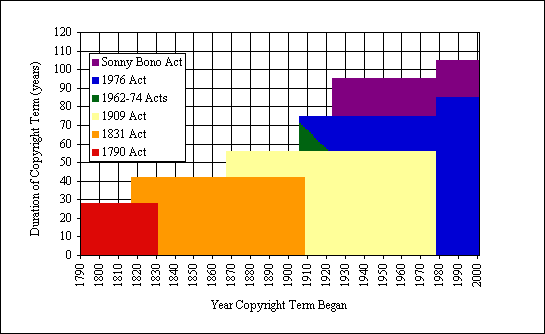
\includegraphics[width=0.5\linewidth]{resources/images/extention_of_us_copyright.png}
    			\caption{Expansion of U.S. copyright term lengths\cite{copyright_term_length_graph_bell}.}
    			\label{fig:ext_us_cop}
			\end{figure}
			
			This implementation of intellectual property law goes against the human rights of access to culture, education and other social and economic rights but is not widely considered so because human rights and intellectual property are regarded as distinct areas of law. By adapting intellectual property law to incorporate human rights, intellectual property law would be reprioritised to promote cultural and scientific progress rather than just reward right owners\cite{handbook_ip_hr_geiger}.
			
			To support this, Dr. Megan Rae Blakely of Lancaster University is looking for assistance in analysing journals and legal instruments for overlap in language. Previously, analysis of the intersection between human rights and intellectual property law has been limited to more manual case-by-case methods. Supplying a more systematic method using natural language processing that can cope with large amounts of data would give concrete evidence of the relationship between human rights and intellectual proeprty. 
		\subsection{Aims and Objectives}
			In the early stages of the project, the following requirements for the project were established:
			\begin{itemize}
				\item A simple Graphical User Interface which allows for input of law journals and treaties PDF form.
				\item A visualisation of all inputted PDF documents with $x$-axis as time; $y$-axis as the intent of the document toward human rights to intellectual property; and $z$-axis as the measure of the extent to which statute protects the owner or the user.
				\item A code base written well enough for any future researcher to easily understand.
			\end{itemize}
			Over the course of the literature review, section \ref{sec:litrev}, I will review past literature in order to find the best methods to achieve each of these requirements.
		\subsection{Added Value}
			The originality of the project stems from its application of natural language processing methods in this domain, rather than the natural language processing methods used, as will be discussed in section \ref{sec:litrev}. Therefore, the added value will come in optimising the techniques used for the application, for example, finding the most appropriate visualisation to illustrate the findings.
			\newpage
		\subsection{Scope}
			Abc
		\subsection{Structure of Literature Review}
			Abc
	\section{Literature Review} \label{sec:litrev}
		\subsection{Definitions}
			Abc
		\subsection{Natural Language Processing Techniques}
			Abc
		\subsection{Graphical Representation Techniques}
			Abc
		\subsection{User Interface}
			Abc
	\section{Preliminary Investigation}
		\subsection{Preliminary Investigation}
			Abc
	\section{Project Plan}
		\subsection{Timeline}
			Abc
		\subsection{Evaluation}
			Abc